\documentclass{article}

% Language setting
% Replace `english' with e.g. `spanish' to change the document language
\usepackage[english]{babel}

% Set page size and margins
% Replace `letterpaper' with `a4paper' for UK/EU standard size
\usepackage[letterpaper,top=2cm,bottom=2cm,left=3cm,right=3cm,marginparwidth=1.75cm]{geometry}

% Useful packages
\usepackage{amsmath}
\usepackage{graphicx}
\usepackage{todonotes}
\usepackage[colorlinks=true, allcolors=blue]{hyperref}

\title{Rock Implementation of an On-Board Terrain Classifier based on Proprioceptive Sensor Data for a Planetary Rover}
\author{
Dominguez. Raul \and Kuhr, Lennart \and Babel, Jonathan
}

\begin{document}
\maketitle

%\begin{abstract}

%\end{abstract}

\section{Introduction}

\todo[inline]{Contact Giulio Reina in case he and someone else from his team wants to be included as authors}

% Introduction main motivation and main idea of the paper explain in detail the implementation of a SMV-based proprioceptive terrain classifier
Automated terrain awareness, the correct modeling of the surfaces transited by a rover and its’ classification, is a key factor for successful navigation. 
\todo[inline]{more on motivation, why is this important? how will it be used by the navigation stack... Problems in missions due to not having this}
In this publication a software component implementation that is capable of classifying the traversed terrain type based on proprioceptive sensor data is presented. 
The component uses a Support Vector Machine (SVM) algorithm \cite{vapnik1992,cristianini2000} in its core and it is integrated into the software control architecture of the hybrid locomotion rover SherpaTT \cite{cordes2018}, such that it can be executed sufficiently fast during navigation. 
The functionality has been integrated using the framework Robotic Construction Toolkit (Rock).
One of the main challenges addressed by the middleware component is to generate online from the multifrequency datastreams, matrices of synchronous sample values for classification.

%During the traverse the terrain classifier component uses proprioceptive sensor data -force torque sensors and joints- and dataproducts -acceleration estimates- to classify between the three terrain types.
% Background and approach
During navigation the terrain classifier component uses force torque sensors, joints data and body acceleration estimates to classify the surface into one of three terrain types: \emph{sand, compact sand} and \emph{concrete}.
The three terrain types represent distinct classes of surfaces characterized by its deformability and fiction properties but are hard to identify with exteroceptive sensors since they are visually similar.
To achieve a better classification performance as well as a more in depth characterization of the surface patches, a feature calculation process is performed.
The computed features estimate physical properties such as mechanical power, electrical power, friction coefficients and speed deviation. 
For all of these feature, a statistical correspondent (mean, variance, skewness and kurtosis) is computed. 
Finally, to reduce the dimensionality of the inputs for the classifier, the identification which of the calculated features and direct inputs are the most valuable for the classification is needed.  
These feature selection process was done using the WB index and the Pearson Coefficient as detailled in \cite{Dimastrogiovanni2020}. 

% Challenges
In order to allow other onboard components to utilize the classification results (e.g. to improve the navigation), the results need to be available at a fast enough pace so that the classification results correspond to the currently traversed surface. 
Likewise, the loss of data samples due to full queues on the input of the processing components must be avoided. 
In Figure \ref{fig:overview} a diagram presents the implementation approach.

\begin{figure}
\centering
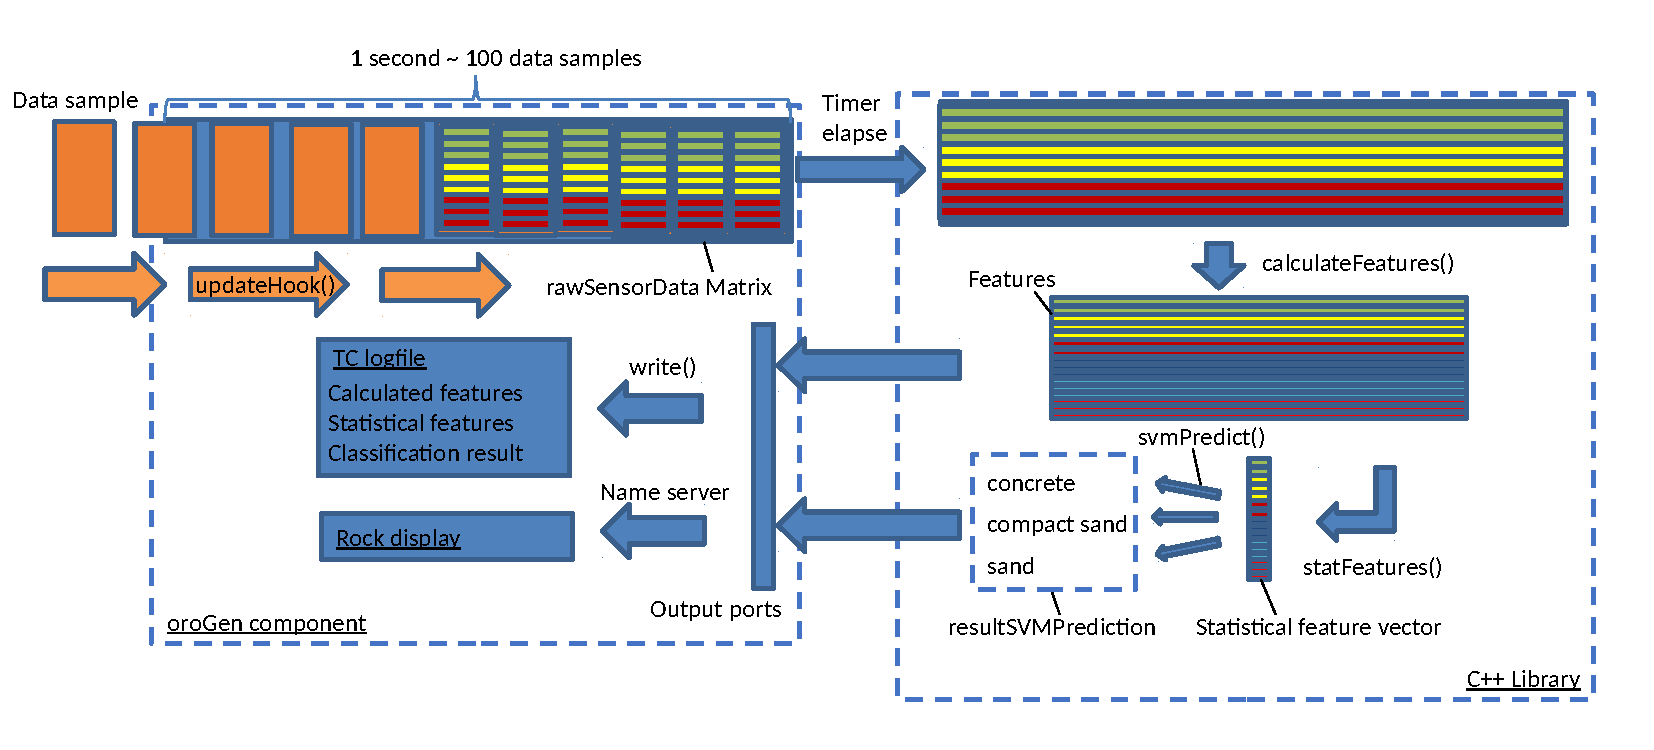
\includegraphics[width=\textwidth]{../figures/OverviewTC2.pdf}
\caption{\label{fig:overview}Overiview of the terrain classifier library and Rock integration.}
\end{figure}

% The SVM model training software is implemented to enable the use of a variable constellation of logged datasets. Moreover, it can be used to compare both the offline and online classification performance. 

% Evaluation
For the analysis of the classification performance onboard SherpaTT, the results generated during several test traverses were logged and compared with the ones from the training sets.
Several tests were conducted which validated that the developed code can be successfully executed on SherpaTT.
Moreover, the classification performance achieved onboard SherpaTT was identified during tests on terrain that represent at least one of the three terrain type classes.


\bibliographystyle{alpha}
\bibliography{sample}

\end{document}